Z minulých kapitol vyplývá, že se veškeré kognitivní funkce člověka promítají
zároveň do těch fyziologických. Většina studií, které se věnují detekci a
hodnocení kognitivní zátěže však tento širší kontext nebere v úvahu. Díky tomu
je nedostatek systematického porovnávání indexů HRV (viz následující
kapitola~\ref{sec:hrv}), což činí interpretaci a vyhodnocování výsledků
zdlouhavým a sporným. Problémem je také samozřejmě dříve zmíněný nedostatek dat.
Tato kapitola slouží k zasazení úlohy této práce do širšího obrazu a zároveň pro
zdůraznění důležitosti problematiky samotné. 

V současné době existuje mnoho studií, které vypovídají o tom, že parasympatický
neboli vagový tonus, souvisí s psychologickými a behaviorálními proměnnými i
zdravotním stavem. Studie například odhalily velký počet konzistentních
zjištění, která ukazují, že jedinci s vyšší variabilitou srdeční frekvence mají
větší schopnosti v oblasti regulace emocí~\cite{Appelhans_Luecken_2006,
Butler_Wilhelm_Gross_2006,Ingjaldsson_Laberg_Thayer_2003,Lane_2008,
Melzig_Weike_Hamm_Thayer_2009, Thayer_Brosschot_2005} a dosahují lepších
výsledků v kognitivních úkolech zahrnujících pozornost, pracovní paměť a
inhibiční kontrolu~\cite{Thayer2009,Hansen_Johnsen_Thayer_2003,
Johnsen_Thayer_Laberg_Wormnes_Raadal_Skaret_Kvale_Berg_2003,
Saus_Johnsen_Eid_Riisem_Andersen_Thayer_2006}. Pokud bychom kategorizovali HRV
pouze na dvě úrovně, vyšší a nižší, tak lze s postupem let pozorovat množství
poznatků z hlediska prognostického významu:
\begin{itemize}
    \item \textbf{vyšší HRV} --- \emph{lepší regulace glukózy, lepší funkce osy
              hypotalamus-nadledviny-hypofýza (HPA), snížení zánětu a snížení rizika
              mrtvice, kardiovaskulárních onemocnění a úmrtnosti ze všech
              příčin}~\cite{Brosschot_Thayer_2007,Liao_Carnethon_Evans_Cascio_Heiss_2002,Thayer_Fischer_2009,Thayer_Lane_2007}
    \item \textbf{nižší HRV} --- \emph{afektivní poruchy, deprese a úzkost,
              špatná kardiovaskulární kondice, vyšší riziko infarktu, zvýšená kognitivní
              zátěž}~\cite{Gorman_Sloan_2000,Kemp_Quintana_2013,Kemp_Quintana_Felmingham_Matthews_Jelinek_2012}
\end{itemize}

\begin{figure}[!htb]
    \begin{center}
        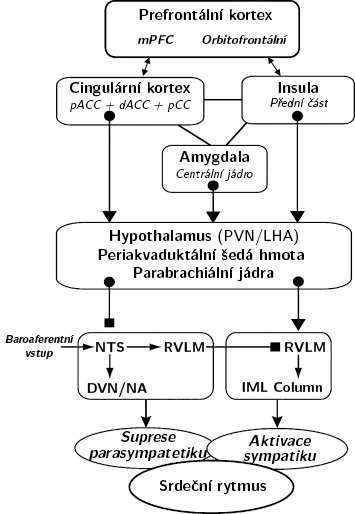
\includegraphics[width=0.9\linewidth]{figures/neurovisceral1}
        \caption{\textbf{(A)} Složené schéma znázorňující dráhy, kterými může
        prefrontální kůra ovlivňovat řízení srdeční frekvence; \textbf{(B)}
        Jádrové oblasti \gls{CAN}, jak je odhalila konjunkční
        analýza\protect\footnotemark\ autonomních modulačních oblastí ve třech
        kategoriích úkolů (barevně označeny). L, levá strana; P, pravá strana
        (Upraveno a převzato z~\cite{gianaros2008,Beissner2013})}
        \label{fig:neurovisceral_diagram}
    \end{center}
\end{figure}

\footnotetext[\thefootnote]{Společné testování více účinků u jednoho subjektu
využitím \gls{fMRI}.}

Objasnění pozorovaných vztahů mezi \gls{HRV} a psychologickými/behaviorálními
proměnnými může v rámci mentálního a fyziologického stavu jedince zlepšit
porozumění a praktickou využitelnost nejen v medicíně. Model
\enquote{\emph{neuroviscerální integrace}} (\gls{NVI}), který v roce 2000
navrhli Thayer a Lane~\cite{Thayer_Lane_2000}, je pokusem o integraci poznatků o
mentálních stavech, autonomních funkcích a zdravotních výsledcích do jednotného
rámce, jehož středobodem je \enquote{\emph{centrální autonomní síť}} (\gls{CAN})
v mozku. \gls{CAN} je síť vzájemně propojených oblastí mozkových
struktur~\cite{Thayer_Lane_2009}. Hlavní části této sítě ukázali pomocí
experimentu Beissner et al.~\cite{Beissner2013} (viz
Obr.~\ref{fig:neurovisceral_diagram}B).

Na diagramu~\ref{fig:neurovisceral_diagram}A lze vidět prefrontální, cingulární a
insulární kůru, jež tvoří propojenou síť s obousměrnou komunikací s amygdalou.
Amygdala je pod tonickou inhibiční kontrolou prostřednictvím prefrontálních
vagových drah k interkalárním buňkám v amygdale. Aktivace centrálního jádra
amygdaly (\gls{CeA}) inhibuje jádro solitárního traktu (\gls{NTS}: plný
čtverec), které následně inhibuje inhibiční vstupy kaudálního ventrolaterálního
medulárního jádra (\gls{CVLM}) do rostrálního ventrolaterálního medulárního
jádra (\gls{RVLM}) sympatoexcitačních neuronů (plný čtverec) a současně inhibuje
vagové motorické neurony v nucleus ambiguus (\gls{NA}) a dorzálním vagovém
motorickém jádru (\gls{DVN}). Kromě toho může CeA přímo aktivovat
sympatoexcitační neurony v RVLM~\cite{gianaros2008}.

\begin{figure}[!htb]
    \begin{center}
        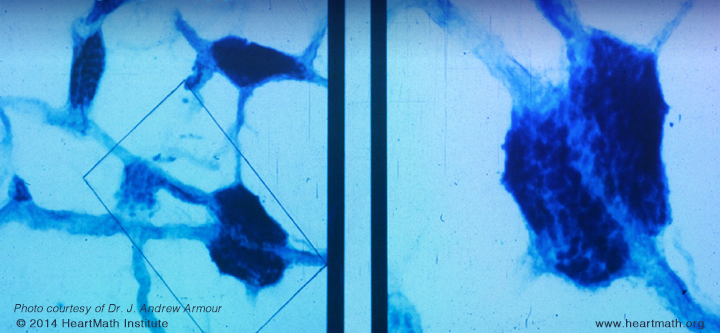
\includegraphics[width=1\linewidth]{figures/cardiac_ganglia}
        \caption{Mikroskopický obraz propojených vnitřních srdečních ganglií v
            lidském srdci. Tenké, světle modré struktury jsou vícenásobné axony,
            které ganglie propojují (Převzato z~\cite{Shaffer2014} se
            souhlasem HeartMath Institutu)}
        \label{fig:cardiac_ganglia}
    \end{center}
\end{figure}

Centrální autonomní síť, tvořena pregangliovými sympatickými a parasympatickými
neurony, inervuje srdce prostřednictvím hvězdicových ganglií a n. vagus. Vlivy
těchto drah na sinoatriální uzel (\gls{SA}) jsou hlavním faktorem určujícím
\gls{HRV}. Vzhledem k rozsáhlým aferentním informacím této autonomní sítě se
promítá úroveň integrace mezi periferním a centrálním nervovým systémem do
\gls{HRV} a poskytuje kontextově specifickou regulaci srdce. Změny autonomních
funkcí, zejména v kognitivních a afektivních souvislostech, odrážejí především
vagový vliv, protože časové měřítko změn tonu sympatiku je relativně pomalejší
než u tonu parasympatiku~\cite{Thayer_Lane_2009,Thayer2009}.

Obrázek~\ref{fig:neurovisceral_diagram}A znázorňuje dráhy, které umožňují
prefrontální kůře regulovat srdeční frekvenci a její variabilitu. \gls{ANS} má
jak tonickou excitační, tak inhibiční kontrolu nad \gls{HR}, kterou může
modulovat frontální kůra prostřednictvím \gls{CeA}. To umožňuje přesnou regulaci
variability srdečního rytmu, která na srdeční úrovní probíhá pomocí
intrakardiálních neuronů (viz Obrázek~\ref{fig:cardiac_ganglia}). Prefrontální
kůra rovněž vykonává tonickou inhibiční kontrolu nad těmito obvody, jak dokládá
inverzní korelace mezi aktivitou ventromediálního prefrontální a orbitofrontální
kortexu a úrovní kožní vodivosti během výchozího stavu mozku\footnote{Základní
stav fyziologického mozku dospělého člověka z hlediska frakce extrakce kyslíku z
mozku neboli OEF~\cite{Raichle2001}.}. To podporuje současný \gls{NVI} model a je
v souladu s pozorováním, kde tyto oblasti jsou deaktivovány během kognitivních
úkolů při současném zvýšení hladiny kožní
vodivosti~\cite{Nagai2004,Raichle2001,Thayer_Lane_2009}.

Souhrnně lze říci, že \gls{NVI} model integruje podstatu periferních
fyziologických změn vlivem specifických mozkových struktur do jednotného
frameworku, který se tyto adaptivní pochody snaží vysvětlit. Podle Thayera a
Lanea~\cite{Thayer_Lane_2000} je tento framework spojen s psychologickými a
fyziologickými procesy prostřednictvím kortiko-subkortikálního neuronálního
okruhu, který lze indexovat pomocí \gls{HRV}. Prefrontální kůra může inhibovat
podkorové struktury, což umožňuje organismu účinně reagovat na požadavky
prostředí~\cite{Thayer_Lane_2009}. Model \gls{NVI} představuje a popisuje
víceúrovňovou funkční strukturu vagové kontroly, jejíž kompletní rozbor ale
přesahuje rozsah této práce. Jednotlivé úrovně dokládají důkazy o souvislosti
mezi \gls{HRV} a fyziologickou, afektivní a kognitivní regulací. Zbytek kapitoly
je proto věnován pouze souhrnu kognitivní regulace. Důkladně byl \gls{NVI} model
rozebrán v literatuře~\cite{Smith_Thayer_Khalsa_Lane_2017,Thayer2009,Thayer_Lane_2009}.

\subsection{Kognitivní regulace}
Schopnost regulovat pozornost a potlačovat nežádoucí reakce (negativní afektivní
stavy) je nezbytná pro přizpůsobení se například právě \gls{ICE} prostředí.
Prefrontální korová aktivita je důležitá pro úkoly vyžadující pracovní paměť,
trvalou pozornost, inhibici chování a mentální
flexibilitu~\cite{Thayer_Lane_2009}. Předchozí studie prokázaly, že jedinci s
vyšší klidovou \gls{HRV} dosahovali lepších výsledků při řešení úkolů (n-back
test, Stroopův test) vyžadujících exekutivní funkce než jedinci s nižší klidovou
\gls{HRV}~\cite{Hansen_Johnsen_Thayer_2003,
Johnsen_Thayer_Laberg_Wormnes_Raadal_Skaret_Kvale_Berg_2003}. Stres může také
zhoršovat kognitivní funkce, přičemž jedinci s nižší klidovou variabilitou
vykazovali horší výkonnost při řešení určitých úkolů, kde byli vystaveni
ohrožení a také větší reakci kortizolu na mírné kognitivní výzvy, které
přetrvávaly i v období zotavení, ve srovnání s jedinci s vysokou klidovou
\gls{HRV}~\cite{Thayer_Lane_2009}.

Saus et al.~\cite{Saus_Johnsen_Eid_Riisem_Andersen_Thayer_2006} ukázali na
realističtějších scénářích zahrnující příslušníky policie, kteří plnili úkoly ve
virtuální realitě, že jedinci s vyšší klidovou \gls{HRV} vykazovali větší
situační povědomí a lepší výkon v plnění úkolu. Kromě toho byl tento krátký
tréninkový program spojen s méně významným snížením \gls{HRV} během plnění
úkolu, což naznačuje snížení mentální zátěže. Tyto výsledky naznačují, že
jedinci s vyšší klidovou \gls{HRV} jsou lépe vybaveni pro plnění úkolů, které
zahrnují exekutivní a inhibiční funkce, a to jak v laboratorním, tak v reálném
prostředí. Navíc naznačují, že trénink může ovlivnit variabilitu srdečního rytmu
a kognitivní výkon.